\subsection{Image Processing}
%Beholde
The use of a camera as a sensor has many advantages in technical applications. It can be effectively used for identifying environmental variables for many applications within the line of sight, and is used more and more frequently in autonomous applications such as self-driving cars. The vast amount of information present in a digital image can be processed, and useful information about the environment can be extracted. \\

For instance, in a self-driving car application, one might be interested in determining the size and location of other cars on the road. The subject of image processing is a topic used in many automation applications, and the theory presented in this section can be used for many different applications.\\
%---

%Endre
I will in the following section represent the fundamental underlying theory of edge detection and edge linking in digital image processing, and present which method I use in my project. I will also present some initial image processing techniques done to the image to make it easier to extract edges, such as smoothing. The implementation in Matlab will also be presented where all the steps and different edge detection model results are displayed, to select the best one for my application.

\subsubsection{Edge Detection}
%Endre litt, se i perpektiv av det jeg har gjort
A powerful tool to use when trying to identify the characteristics of a the environment is edge detection. Edge detection is based on detecting sharp, local changes in intensity in an image. At a fundamental level, abrupt, local changes in intensity can be detected by using derivatives, where first- and second order derivatives are the most used \cite{g}. \\

Figure \ref{fig:derivatives} illustrates the differences between the intensity response of the first- and second order derivatives on an edge with a ramp response.

\begin{figure}[h]
  \centering
  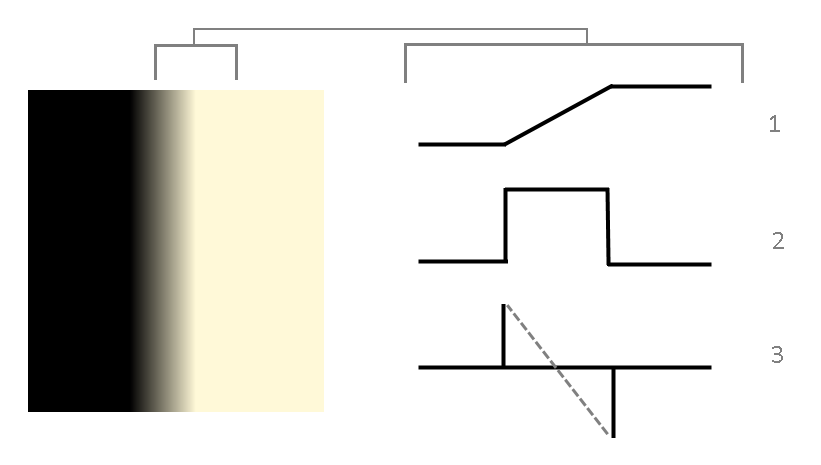
\includegraphics[width=0.8\textwidth]{fig/derivatives}
  \caption{(1) Horizontal intensity profile. (2) First derivative. (3) Second derivative with zero crossing}
  \label{fig:derivatives}
\end{figure}

\subsubsection{Edge Detection methods based on first derivatives}
As mentioned previously, edges are characterized as a change in intensity in an image. Digital images are discrete, therefore we have to use an approximation of the first derivative with the requirements that; (1) it must be zero in areas of constant intensity, (2) it must be nonzero at the onset of an intensity step or ramp, and that (3) it must be nonzero at points along an intensity ramp\cite{g}. It is important to note that most edges in an image does not change its value immediately, but tends to change more gradually, like a ramp-function. Our requirements covers this, where the derivative must be non-zero along an intensity ramp.\\
We first consider the one-dimensional function $f(x)$, we approximate by Taylor expansion about $x$ of $f(x+\Delta x)$, where we let $\Delta x = 1$, and keep the linear terms:
\begin{align}
    \frac{\partial f}{\partial x} = f'(x) = f(x +1) - f(x)
\end{align}
We used the partial derivative here because the image is a function of two variables. We approximate the the derivative by Taylor expansion in the $y$ dimension just like we did above:
\begin{align}
\frac{\partial f(x,y)}{\partial x} = f(x+1,y)-f(x,y) = g_x\\
\frac{\partial f(x,y)}{\partial y} = f(x,y+1)-f(x,y) = g_y
\end{align}
A powerful tool in edge detection is to define the gradient, $\nabla f$ as
\begin{align}
\nabla f \equiv grad(f) \equiv 
\begin{bmatrix}
g_x \\
g_y
\end{bmatrix}
= 
\begin{bmatrix}
\frac{\partial f}{\partial x}\\
\frac{\partial f}{\partial y}
\end{bmatrix}\\
M(x,y) = \sqrt[]{g_x^2 +x_y^2}
\label{eq:magnitude}
\end{align}
Where the $\nabla f$ vector gives us information about the edge strength as well as the direction of the greatest rate of change of $f$ at location $(x,y)$.\\

The direction of the edge can be expressed as:
\begin{align}
\alpha(x,y) = \arctan(g_y/g_x)
\label{eq:direction}
\end{align}

Obtaining the gradient of an image involves calculation the partial derivatives $\frac{\partial f}{\partial x}$ and $\frac{\partial f}{\partial y}$ at every location of the pixels in the image. In order to do this we use spatial filtering in the image (also known as masking). The process of spatial filtering consists of moving a filter mask from point to point in an image, and calculating the filter response of the original image at each point $(x,y)$ in the image. The filter values are pre-defined and characteristics of the filter can be modified in order to achieve different improvements in an image such as image enhancement.\\

We want to look for edges in two dimensions; x and y direction, thus the most used edge detection algorithms use 2D spatial filters to find edges. A general 3x3 spatial filter mask can be represented as a table of intensity values $z_i$ as illustrated in Table \ref{spatial}.
\begin{table}[h]
\centering
\caption{General 3x3 Spatial Filter Mask}
\label{spatial}
\begin{tabular}{|l|l|l|}
\hline
$z_1$ & $z_2$ & $z_3$\\ \hline
$z_4$ & $z_5$ & $z_6$\\ \hline
$z_7$ & $z_8$ & $z_9$\\ \hline
\end{tabular}
\end{table}



\paragraph{Roberts Method}

\begin{table}[h]
\centering
\caption{Roberts Spatial Filter}
\begin{tabular}{|l|l|}
\hline
-1 & 0 \\ \hline
0  & 1 \\ \hline
\end{tabular}
\quad
\begin{tabular}{|l|l|}
\hline
0 & -1 \\ \hline
1 & 0 \\ \hline
\end{tabular}
\label{roberts}
\end{table}
The Roberts cross-gradient operators are one of the most basic implementations of 2-D masks based on the first derivative, and it registers diagonal differences in the image. The filter is illustrated in Table \ref{roberts}, and can be expressed as solving for the diagonal differences:
\begin{align*}
g_x = \frac{\partial f}{\partial x} = (z_5-z_1)\\
g_y = \frac{\partial f}{\partial y} = (z_4 - z_2)
\end{align*}
This method fulfills the requirements set on the approximation of first derivatives. This method is relatively simple conceptually, but the mask size of 2x2 is not as useful as masks symmetrical about the center point; the smallest being the 3x3 mask. 

\paragraph{Prewitt Method}

\begin{table}[h]
\centering
\caption{Prewitt Spatial Filter}
\begin{tabular}{|l|l|l|}
\hline
-1 & -1 & -1 \\ \hline
0  & 0 & 0 \\ \hline
1 & 1 & 1 \\\hline
\end{tabular}
\quad
\begin{tabular}{|l|l|l|}
\hline
-1 & 0 & 1 \\ \hline
-1 & 0 & 1 \\ \hline
-1 & 0 & 1 \\ \hline
\end{tabular}
% \quad
% \begin{tabular}{|l|l|l|}
% \hline
% 0 & 1 & 1 \\ \hline
% -1 & 0 & 1 \\ \hline
% -1 & -1 & 0 \\ \hline
% \end{tabular}
% \quad
% \begin{tabular}{|l|l|l|}
% \hline
% -1 & -1 & 0 \\ \hline
% -1 & 0 & 1 \\ \hline
% 0 & 1 & 1 \\ \hline
% \end{tabular}
\label{prewitt}
\end{table}
The Prewitt method, as well as other odd-numbered masks take into account the values around the point $(x,y)$ and thus giving us more information about the direction of an edge. The Prewitt spatial filter is illustrated in Table \ref{prewitt}, where the first filter is for detecting horizontal changes, and the second for detecting vertical changes in intensity in an image. It can be expressed as:
\begin{align*}
g_x = \frac{\partial f}{\partial x} = (z_7+z_8+z_9)-(z_1+z_2+z_3)\\
g_y = \frac{\partial f}{\partial y} = (z_3 + z_6+z_9) - (z_1+z_4+z_7)
\end{align*}
Here the $g_x$ estimates the derivative by the difference between the first and third row, while $g_y$ estimates the derivative by the difference between the first column and the third column. This filter is relatively easy to implement and not very computationally demanding, but is particularly sensitive to noise.

\paragraph{Sobel Method}
\begin{table}[h]
\centering
\caption{Sobel Spatial Filter}
\begin{tabular}{|l|l|l|}
\hline
-1 & -2 & -1 \\ \hline
0  & 0 & 0 \\ \hline
1 & 2 & 1 \\\hline
\end{tabular}
\quad
\begin{tabular}{|l|l|l|}
\hline
-1 & 0 & 1 \\ \hline
-2 & 0 & 2 \\ \hline
-1 & 0 & 1 \\ \hline
\end{tabular}
\label{sobel}
\end{table}
A slight variation of the Prewitt filter is the Sobel filter, which places a weight of 2 in the center coefficients. This is illustrated in Table \ref{sobel}, and can be expressed as:
\begin{align*}
g_x = \frac{\partial f}{\partial x} = (z_7+2z_8+z_9)-(z_1+2z_2+z_3)\\
g_y = \frac{\partial f}{\partial y} = (z_3 + 2z_6+z_9) - (z_1+2z_4+z_7)
\end{align*}
Using 2 in the center coefficients provides smoothing in the image. This means that the Sobel filter has better noise suppression than the Prewitt filter. Computationally, the Sobel operator is a little more demanding, but it is still preferred over the Prewitt operator due to its noise suppression properties.

\subsubsection{Edge Detection methods based on the second derivative}
The requirements we set on the approximation of the second order derivative is similar to that set on the first order derivative. The only difference is that we now only require the second order derivative to be non-zero at the onset and end of a ramp in intensity value. This means that the first order derivative methods will create "thicker" edges since its non-zero along the whole ramp, while the second order derivative methods will lead to "thinner" edges, since the values are non-zero only at the beginning and the end of a ramp.

\paragraph{Laplacian of Gaussian method (LoG}
One of the fundamentals in edge detection is the fact that intensity changes (edges) in an image is not independent of image scale. The LoG algorithm, proposed by Marr and Hildreth \cite{mh}, has two features distinct features; (1) it approximates the first- and second order derivative at every point in the image, and (2) it is capable of being tuned to work on any scale. Large operators would detect blurry edges, and small operators would be used to detect sharper and fine details in the image. \\

For this task they proposed that the second derivative of a Gaussian filter $\nabla^2G$ could be used. $\nabla^2$ is the Laplacian operator and can be expressed as:
\begin{align}
\nabla^2 = \frac{\partial^2}{\partial x^2} + \frac{\partial^2}{\partial y^2}
\end{align}
where G is the 2-D Gaussian function:
\begin{align}
G(x,y) = e^{-\frac{x^2 +y^2}{2\sigma^2}}
\label{gauss}
\end{align}
where $\sigma$ is the standard deviation. The larger the $\sigma$, the greater the smoothing in the image. The expression for $\nabla^2G$ is:
\begin{align}
\nabla^2G = \Bigg[ \frac{x^2+y^2-2\sigma^2}{\sigma^4}\Bigg]e^{-\frac{x^2 +y^2}{2\sigma^2}}
\label{logoperator}
\end{align}
This is called the Laplacian of a Gaussian (LoG). This function is illustrated in Figure \ref{fig:log}. Because of the shape of the function, this is also known as the Mexican hat operator. What we want to do is approximate the shape in Figure \ref{fig:log} in a mask. This is not a unique approximation. A 5x5 approximation mask is illustrated in Table \ref{LoG}. The mask can be of arbitrary size, and one way to generate a mask is by sampling (\ref{logoperator}), and scaling the mask such that it sums to zero. A different way is to sample (\ref{gauss}) to the desired $n\times n$ size and convolve the resulting array with a Laplacian mask \cite{g}. 
\begin{figure}[h]
  \centering
  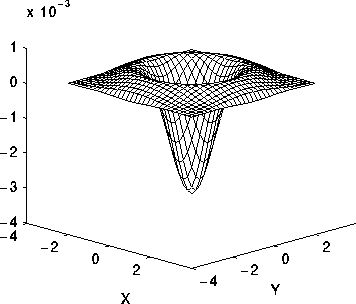
\includegraphics[width=0.7\textwidth]{fig/log}
  \caption{3-D plot of the LoG function $\nabla^2G$}
  \label{fig:log}
\end{figure}
\begin{table}[h]
\centering
\caption{Laplacian of Gaussian spatial filter}
\begin{tabular}{|l|l|l|l|l|}
\hline
0 & 0 & 1   & 0 & 0\\\hline
0 & 1 & 0   & 1 & 0\\\hline
1 & 2 & -16 & 2 & 1\\\hline
0 & 1 & 2   & 1 & 0\\\hline
0 & 0 & 1   & 0 & 0\\\hline
\end{tabular}
\label{LoG}
\end{table}\\

The Laplacian of a Gaussian method can be summarized as:
\begin{enumerate}
\item Filtrate the image with an $n\times n$ Gaussian low-pass filter. This filter is obtained by sampling (\ref{gauss}).
\item Compute the Laplacian of the resulting image from step 1. To compute the Laplacian we can use a simple Laplacian mask made for point detection.
\item Find the zero crossing of the image obtained from step 2.
\end{enumerate}

\paragraph{Canny edge detection method}
A different edge detection algorithm is the Canny method, and is more complex than the Laplacian of Gaussian edge detection algorithm. In general, the Canny method is regarded as superior to most other edge detection algorithms, and is based on three objectives:
\begin{itemize}
\item Low error rate. The algorithm should find all the edges in an image, regardless or orientation. Should be as close as possible to the actual edges.
\item Edge points should be well localized. Detected edges should be close to the actual edges.
\item Single edge point response. Should not return multiple edge points where only a single edge point exist.
\end{itemize}
Similar to the LoG algorithm, the Canny method starts with applying a Gaussian filter to convolve with the image in order to smooth out noise. After this the gradient magnitude (\ref{eq:magnitude}) and direction (\ref{eq:direction}) are calculated:
\begin{align*}
M(x,y) = \sqrt[]{g_x^2 +x_y^2}\\
\alpha(x,y) = \arctan(g_y/g_x)
\end{align*}
After this it applies a non-maximum suppression technique to the gradient magnitude image which thins the edges. This helps suppress all the gradient values to zero except the local maximal, which is the the sharpest change in intensity value, thus fulfilling the objective of giving a single edge point response.\\

The last part of the algorithm is to use double thresholding to determine strong and weak edges. Edges with intensity values below the lowest threshold are suppressed, which is noise in most cases. This is a tuning parameter and needs to be determined empirically. The last step of the algorithm also involves tracking edges and conducting a connectivity analysis to detect and link edges together, where edges that are weak and not connected to strong edges are suppressed.\\
\\
\\
\\

\subsection{Image pre-processing before Edge detection}
There are a number of different techniques and methods one can employ before using an edge detection algorithm to get a better edge detection result.
\subsubsection{Correcting Nonuniform Illumination}
Depending on the lighting conditions in the image, it might be beneficial to correct for nonuniform illumination. This can be done in several ways, but the most normal being estimate the background illumination of the image, inverse it and subtract it from the original image.
\subsubsection{Smoothing}
Smoothing is beneficial to suppress noise in the image. This can be done by applying a Gaussian filter to the image, which described previously in some of the edge detection algorithms. Smoothing is a part of some of the edge detection algorithms, which is designed to suppress noise.
\subsubsection{Increase contrast}
Increasing contrast can help in the detection of edges in an image. This is done by saturating the top and bottom $1\%$ of intensity values in the image. In the implementation described later in the report, this is utilized to improve the edge detection algorithm.
\subsubsection{Re-sizing}
By re-sizing the image by a scale factor the image will be smoothed. Some edge detection algorithms work better with images that are scaled down and smoothed. This is described later in Section \ref{testing}, and how this affects edge detection and edge linking quality.

\newpage
\subsection{Choice of Edge detection method}
\label{choice}
When comparing and selecting an edge detection method to use for the identification of walls in the maze, we want to identify the algorithm that has the following qualities:
\begin{itemize}
\item Filters noise efficiently
\item Takes advantage of the top of the wall being darker than the rest of the environment
\item The edges are coherent and connected, with no gaps
\end{itemize}
The following algorithms will be implemented and tested in Matlab: Roberts, Prewitt, Sobel, Laplacian of Gaussian and Canny. Each algorithm will be tuned empirically to get the best possible result. In order to test the different algorithms we we can use the following procedure, implemented in Matlab:
\begin{enumerate}
\item Re-size the image by a factor of $0.3$ to simulate a more realistic image sensor. This also provides some marginal smoothing in the image.
\item Convert the image to a gray-scale image
\item Adjust the intensity values in the image such that 1\% of the high and low intensity values are saturated
\item Apply the algorithm on the image
\item Attempt trial-and-error tuning and repeat step 4 as long as the edges of the wall stay connected (no gaps)
\end{enumerate}
Figure \ref{fig:testimage} shows the test image which we are trying to detect edges. This is a high resolution image taken by a Sony IMX377 image sensor \cite{cam} of a small part of a maze. The background in the image is not uniform, and there are also a metal charging station for the Lego robots on the back wall. The algorithm should be able to suppress these characteristics of the image and detect the edges on the wall.
\begin{figure}[H]
\centering
  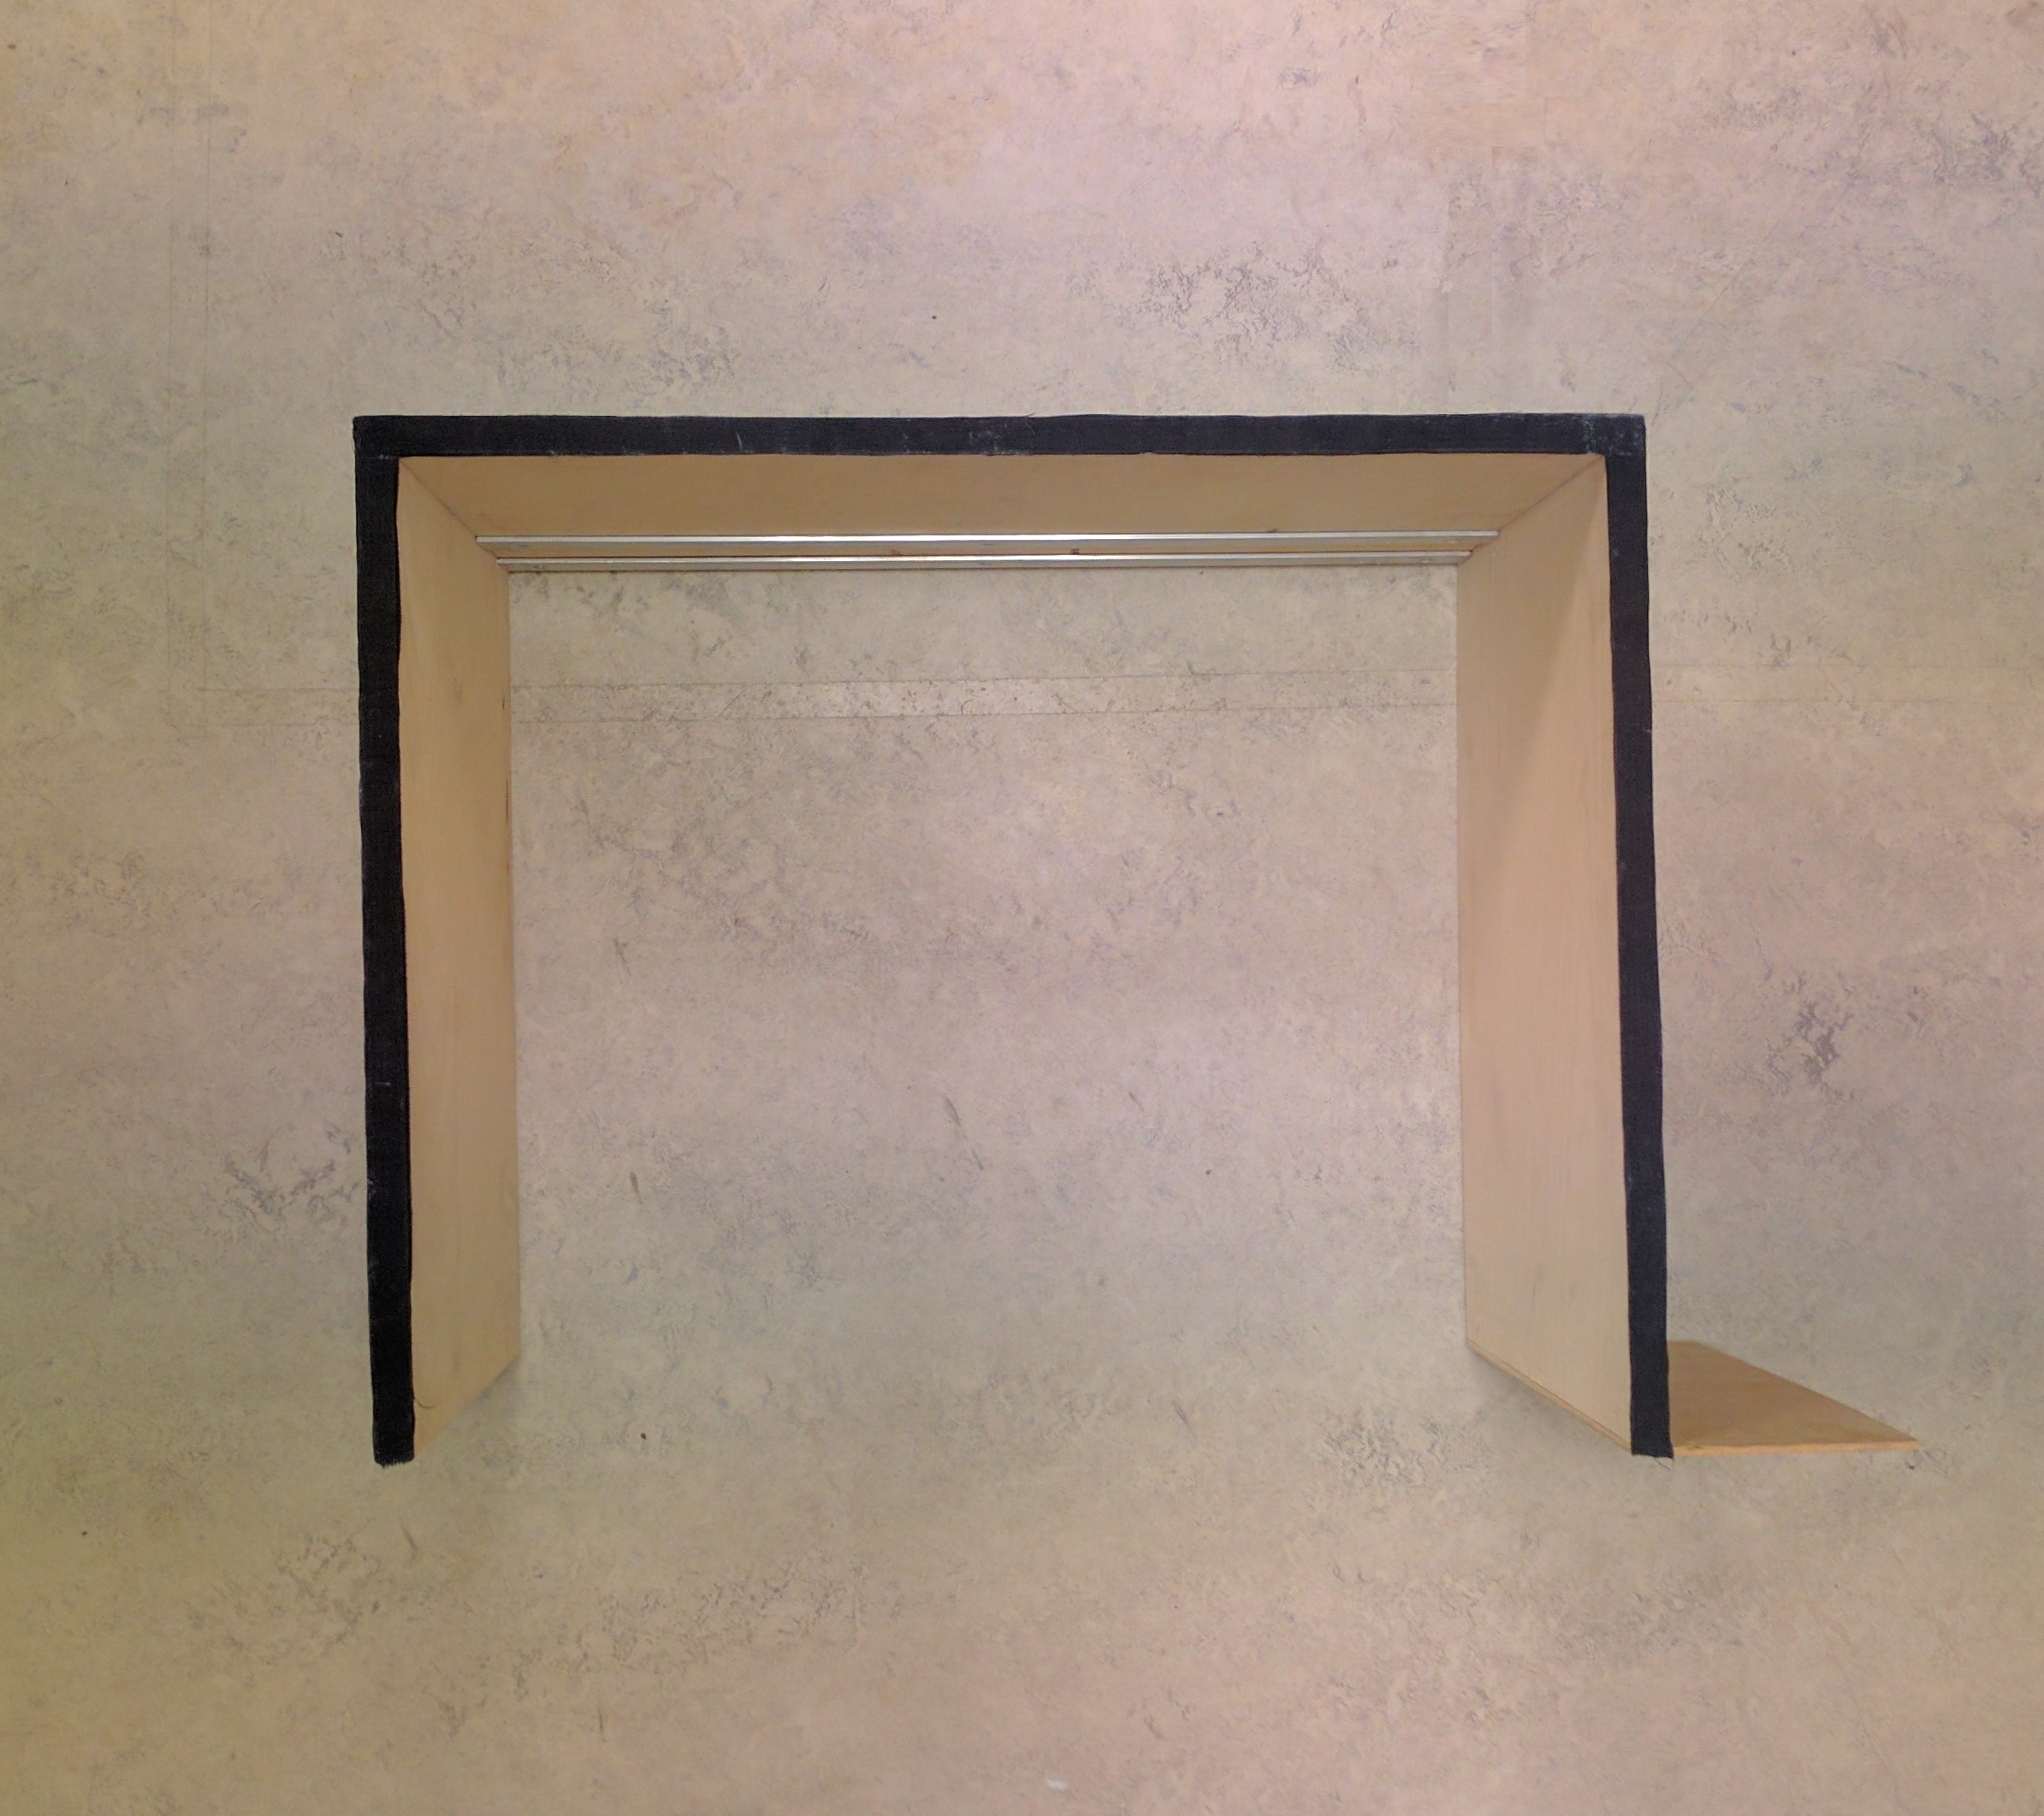
\includegraphics[width=.7\linewidth]{fig/Compare}
  \caption{Original test image. \texttt{Compare.jpg}}
  \label{fig:testimage}
\end{figure}
\begin{figure}[H]
  \centering
  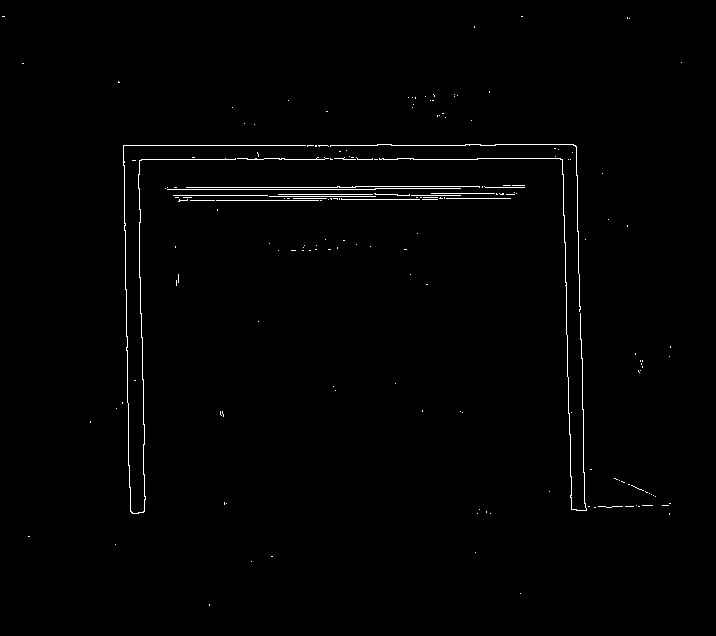
\includegraphics[width=.7\linewidth]{fig/Roberts}
  \caption{Roberts method}
  \label{fig:robertstest}
\end{figure}
\begin{figure}[H]
  \centering
  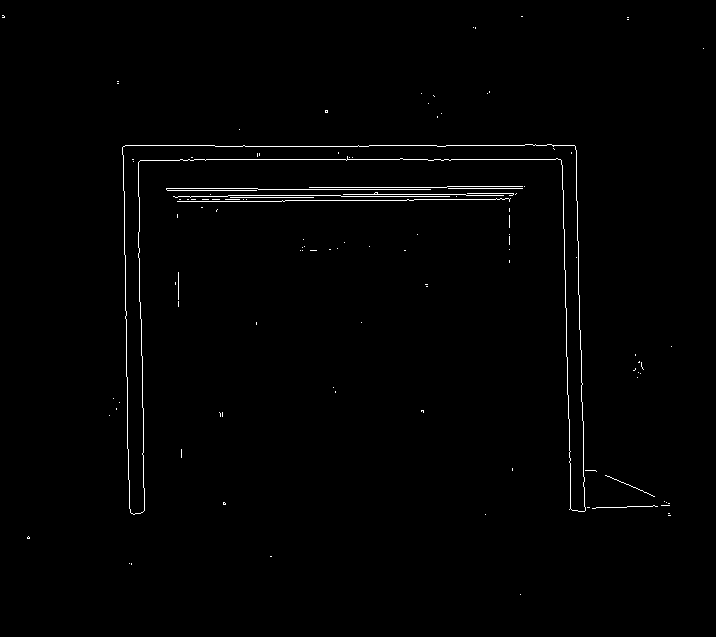
\includegraphics[width=.7\linewidth]{fig/Prewitt}
  \caption{Prewitt method}
  \label{fig:prewitttest}
\end{figure}
\begin{figure}[H]
  \centering
  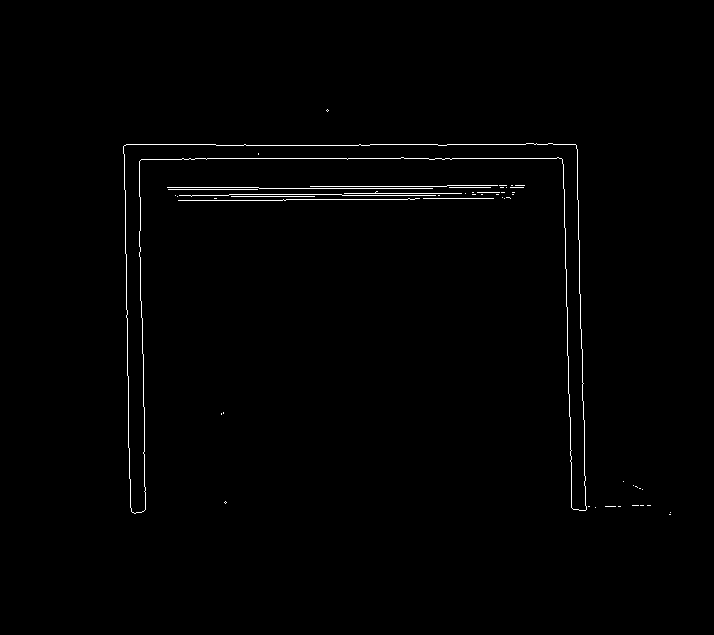
\includegraphics[width=.7\linewidth]{fig/Sobel}
  \caption{Sobel method}
  \label{fig:sobeltest}
\end{figure}
\begin{figure}[H]
  \centering
  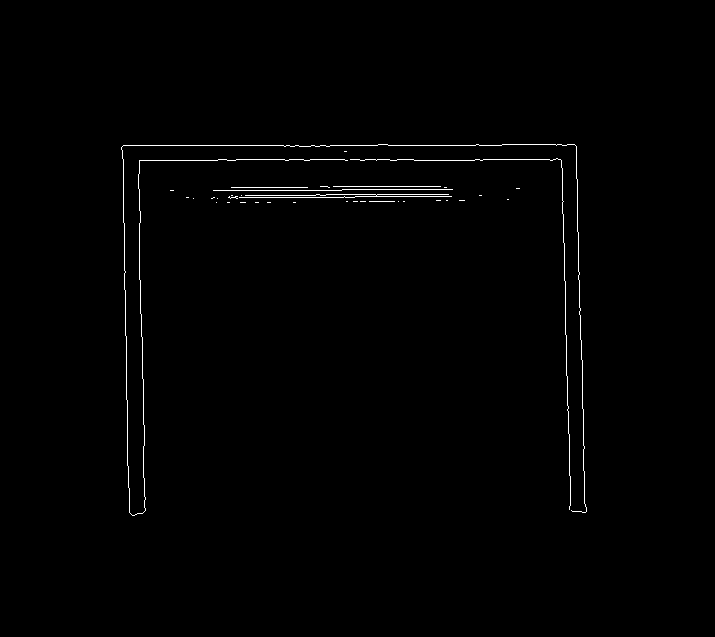
\includegraphics[width=.7\linewidth]{fig/LoG}
  \caption{Laplacian of Gaussian method}
  \label{fig:logtest}
\end{figure}
\begin{figure}[H]
  \centering
  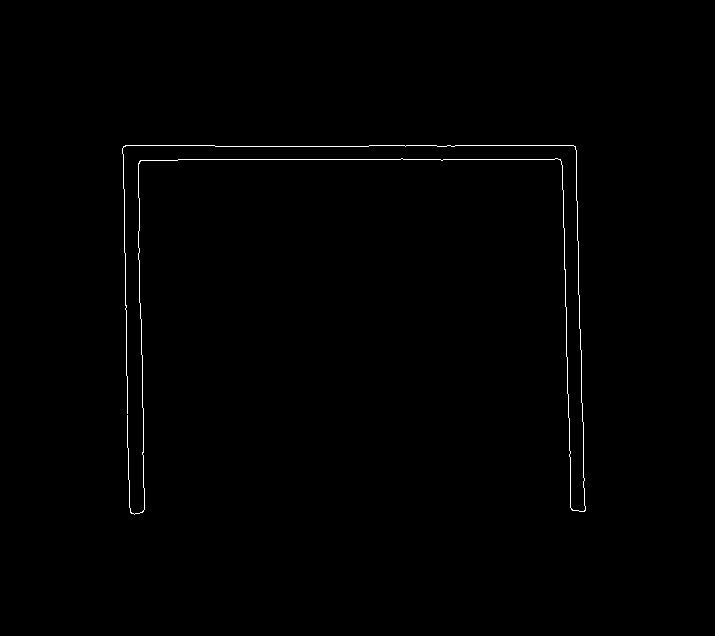
\includegraphics[width=.7\linewidth]{fig/Canny}
  \caption{Canny method}
  \label{fig:cannytest}
\end{figure}
\subsubsection{Choice}
Figure \ref{fig:testimage} to \ref{fig:cannytest} displays the results from the applying the different algorithms on the same image. The most vital part of this test is to determine if any of the algorithms can identify the edges on top of the wall, while excluding the edge between the wall and the floor, as well as the metal charging plate on the back wall. All the algorithms based on the first-order derivative has some problems with noise, and they also detect both the metal charging plate and the edge between the floor and the wall. In this environment, they are not the preferred option for our application.\\

The last two methods, the Laplacian of Gaussian and the Canny method gives a cleaner image with less noise. The Laplacian of Gaussian algorithm identifies the top part of the wall, but it also identifies the charging plate on the wall. By tuning, the algorithm would experience gaps in the edges of the top wall before the loading plate was suppressed. The Canny method with appropriate tuning does a great job of only detecting the top of the wall, while suppressing all other edges that are not important. The algorithm takes advantage of the top of the wall being darker than the rest of the wall, and moving forward this will be the algorithm of choice.

\subsection{Edge Linking}

After the edge detection algorithm has been applied to the image, we ideally have detected all the edge pixels in the image perfectly. Most of the time, this is not the case. The edge detection is therefore followed up by edge linking, where we attempt to assemble edge pixels into meaningful edge segments. Since actual edges will have the property of being fully or partly connected straight lines, noise in the image will naturally be suppressed and not detected. 

\subsubsection{Hough Transform}\label{ch:hough}
The Hough transform is a global processing method of edge linking \cite{hough}.  Considering a point $(x_i,y_i)$ in the xy-plane, we can describe infinitely many lines running through this point as $y_i = ax_i + b$ for any $a$ and $b$. We can rewrite this as $b = -ax_i + y_i$, and consider the ab-plane, which is known as the parameter space. This gives an equation for a single line for a single xy-pair $(x_i,y_i)$. A different xy-pair $(x_j,y_j)$ also has a line expressed in parameter space $b = -ax_j + y_j$, and if the lines are not parallel, the lines will intersect at a point $(a',b')$. $a'$ is the slope, and $b'$ is the intercept of the line containing both $(x_i,y_i)$ and $(x_j,y_j)$. The points on this line will have lines in the ab-plane that intersects at $(a',b')$.\\

One fundamental problem representing lines on the form $y = ax + b$ is that $a$ approaches infinity as the line gets closer to vertical. It is therefore beneficial to represent the lines as:
\begin{align*}
x\cos{\theta} + y\sin{\theta} = \rho
\end{align*}
This is a transformation to the $\theta\rho$-plane, which is very similar to that of the ab-plane. $(\theta',\rho')$ corresponds to the line that passes through both $(x_i,y_i)$ and $(x_j,y_j)$. When $(\theta',\rho')$ has a high concentration of curves passing through it, it indicates that these curves are a part of a connected line in the xy-plane. The Hough transform algorithm can be expressed as\cite{g}:
\begin{enumerate}
\item Use edge detection on an image and obtain a binary image edge image
\item Transform image to the $\theta\rho$-plane
\item Count and examine lines intersecting in the $\theta\rho$-plane
\item Determine the lines based on number of intersects in $(\theta',\rho')$
\end{enumerate}
By using Hough transform the length of each wall segment can be extracted in pixel values. This is very important to make us able to map the maze in real-life units.

\subsection{Mapping}
\label{ch:mapping}
The primary goal in this project is to be able to map a maze. Techniques explained previously lays the ground work for how we are able to extract useful information from the image to be used for mapping. In addition to the information extracted by the image, we need some additional information for mapping:
\begin{itemize}
\item Height $H_{tot}$ above ground the image was taken from as well as x-y position
\item The orientation of the image sensor
\item Assume we know the height of the walls $H_w$
\item Information about the image sensor (pixel pitch $p$ and focal length $f$)
\end{itemize}
We also put the following assumptions on the maze and image:
\begin{itemize}
\item The wall height $H_w$ is constant on the entire maze
\item The walls are straight (no curves)
\item The walls are normal to the ground (no angle)
\item The line of sight of the image covers the entire maze (one image sufficient)
\end{itemize}
Figure \ref{fig:mapping} displays the setup and different heights and planes associated with our mapping looking perpendicular to the ground. We can see that the wall plane height $H_p = H_{tot} - H_w$. 
\begin{figure}[H]
\centering
\includegraphics[width=\linewidth]{fig/Mappingsetup}
  \caption{Mapping setup}
  \label{fig:mapping}
\end{figure}
One key insight in this setup is a result of taking the image normal to the ground and wall plane. Looking at Figure \ref{fig:mapping}, we can see that if we used the total height $H_{tot}$ in our calculation, the top of the wall would be projected an error $e$ away from the actual base of the maze. Since we are taking the image normal to the ground, and we know the height of the wall $H_w$, we can move to the wall plane and do our calculations here instead of doing it at the ground plane, thus eliminating the error $e$. We can simply move our projected map a distance $z = -H_w$ after the mapping is done to coincide the top of the wall with the base of the wall.

\subsubsection{Determining the length of the walls}
As mentioned previously, Hough transform gives us the straight line segments of the maze and their respective lengths in pixels are easy to extract. The Hough transform algorithm outputs a list of x-y coordinates in pixels that define the start- and end-point of each detected line segment. To extract the lengths of each line segment we can use:
\begin{align}
\textbf{Length of line} = l_i = \sqrt{(x_{i+1} - x_i)^2 + (y_{i+1} - y_i)^2 }\quad [pixels]
\end{align}
Ground Sample Distance (GSD) can now be used to convert these lengths in pixels to lengths in meters. The length $L$ can be expressed in [m]:
\begin{align}
L_i = l_i \times GSD\quad [m]\\
L_i = l_i \times \frac{p}{fW}H_p\quad [m]
\end{align}
Where $H_p$ is the distance from the optics to the top of the wall and $W$ is the width of the image in pixels. $p$ is the pixel pitch and $f$ is the focal length of the image sensor.  

\subsubsection{Determining the position of the walls}
The information used when finding the length of the walls can be also used to transform the position in the image to their respective real-life position. The Hough transform outputs a list of the start and end position of the line segments in pixels. To transform these values to real life values we need information about the location of the image sensor. When taking the image, we assume we have measurements for the x-y position in the real world of the image sensor. Since we are taking the picture normal to the wall- and ground plane, the x-y position of the image sensor in the real world corresponds to the center of the image.\\

There are several ways to extract and transform the position of the walls from the Hough transform to real-life units. One way is to transform the start- and end point coordinates in pixels of each wall segment to meters with respect to the image center. This can be done by first finding the GSD of the image and after that subtracting the x- and y component of each start- and end point by the x- and y component of the center and multiplying by the GSD.\\

If we have the position of the center $(x_c,y_c)$ and the start- and end point of a line segment $(x_1,y_1)$ and $(x_2,y_2)$ in the image respectively. The position of each of these points relative to the center can be expressed as:
\begin{align}
\textbf{Position of start point} = GSD\times(x_1-x_c, y_1-y_c)\quad [m]\\
\textbf{Position of end point} = GSD\times(x_2-x_c, y_2-y_c)\quad [m]
\end{align}
Since we know the start and end point coordinates in real life units of all wall segments, we have all the information we need to express the characterization of the maze. We assume we know the orientation of the image sensor when the image is taken, giving us a complete characterization of where each wall segment is in the real world. \\

It is important to note that I am not calculating or implementing the orientation of the image sensor when the image is taken. It is assumed we have a measurement of the orientation about an inertial axis in the ground- and wall plane, so that the mapping directly relates to this inertial frame. This means that we require the UAV to measure the attitude when mapping the maze.







